\chapter{随机向量}
\label{chap:random-vectors}

同一个房间里装了两台温度传感器，每台把读数粗分成三档：$0$表示偏低，$1$表示正常，$2$表示偏高。前几章的工具可以分别描述每台传感器：它读“偏高”的概率是多少，读数的平均档位和波动有多大，读数超过某个档位的概率有多小。可是值班人员真正关心的问题常常同时涉及两台：两台同时报“偏高”的机会有多大？第一台读“偏低”时，第二台还可能读“偏高”吗？把两台读数取平均，波动能比一台小多少？

这些问题都在问两个量在同一次观测中怎样共同取值。只知道每台传感器各自的分布，回答不了它们；需要一份记录“哪一对读数以多大概率一起出现”的规律。本章把同时观察的几个随机变量合成一个随机向量，研究这份共同规律包含什么信息，又怎样从中取出常用的部分。

本章分四步展开。第一节建立联合分布，用概率表、联合密度和联合分布函数描述它，并说明怎样取出单个分量的边缘分布，以及为什么反过来不行。第二节讨论联合分布恰好由边缘决定的情形，即独立。第三节用均值向量和协方差矩阵概括联合分布的中心与波动，解释交叉项从哪里来。第四节固定一个变量的取值，重新归一化，得到条件分布、条件均值和全方差公式。

全章以两台传感器的概率表和三角形上的均匀密度为贯穿例子，前者代表离散情形，后者代表连续情形。具体的多元分布模型在第~\ref{chap:multivariate-distributions}章介绍，随机向量经过变换以后的分布在第~\ref{chap:random-variable-transformations}章计算。

\section{联合分布}
\label{sec:rvc-joint}

两台传感器各自的读数规律，第~\ref{chap:random-variables}章已经会写：每台都有一张概率表。要回答“两台同时报偏高”这样的问题，需要的却是读数\emph{对}的概率。这一节先说明几个随机变量怎样放进同一次试验，再用概率表、密度和分布函数记录它们的共同规律，最后从共同规律中取出单个分量的规律。

\paragraph{同一次试验中的几个随机变量}
随机变量是样本空间$\Omega$上的函数：试验给出一个样本点$\omega$，随机变量把它变成一个数。几个随机变量要能“一起取值”，必须定义在同一个$\Omega$上，这样同一个$\omega$同时决定它们全部的值。

掷两颗均匀骰子是最直接的例子。样本空间由$36$个等可能的有序对$(i,j)$组成，$i$是第一颗的点数，$j$是第二颗的点数。令$X$为第一颗的点数，$M$为两颗中较大的点数，即
\[
 X(i,j)=i,\qquad M(i,j)=\max\{i,j\}.
\]
每个样本点同时给出一对值$(X,M)$。事件$\{X=4,\,M=4\}$由第一颗为$4$、第二颗不超过$4$的四个样本点组成，概率是$4/36$；事件$\{X=2,\,M=5\}$只含样本点$(2,5)$，概率是$1/36$。

把$36$个样本点按它们给出的$(X,M)$分组，每组的点数除以$36$，就得到每一对取值的概率，见图~\ref{fig:rvc-dice-map}。表中右下方的空格表示$M<X$的取值对，它们不可能出现，因为较大点数不会小于第一颗的点数。这张表记录的正是“两个量怎样一起取值”。

\begin{BookInlineFigure}
  \centering
  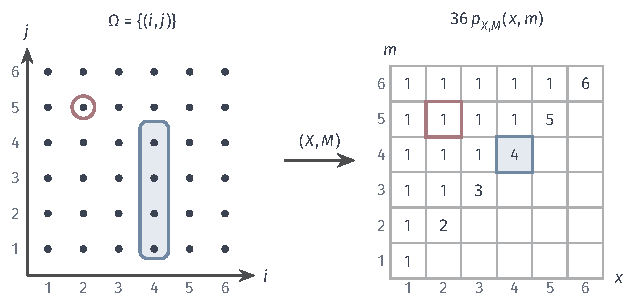
\includegraphics[width=107mm]{figures/07-probability/01-elementary-probability/tikz/rvc-dice-map/figure.pdf}
  \caption{从样本点到联合概率表。左侧是两颗骰子的$36$个样本点，横坐标为第一颗点数$i$，纵坐标为第二颗点数$j$。右侧格子$(x,m)$中的数是满足$X=x$、$M=m$的样本点个数，除以$36$即为概率。蓝框中的四个样本点都给出$(X,M)=(4,4)$，红圈中的样本点$(2,5)$单独给出$(2,5)$；空格的概率为零。}
  \label{fig:rvc-dice-map}
\end{BookInlineFigure}

\begin{definition}[随机向量与联合分布]
\label{def:rvc-random-vector}
设$X_1,\dots,X_d$是定义在同一样本空间$\Omega$上的随机变量。把它们排成列向量
\begin{equation}
 \bm{X}=(X_1,\dots,X_d)^{\top},
 \label{eq:rvc-random-vector}
\end{equation}
称为$d$维\term{随机向量}（random vector）。对$\mathbb{R}^{d}$中的集合$A$，事件$\{\bm{X}\in A\}$由使$\bm{X}(\omega)\in A$的样本点组成；这些事件的概率$\mathbb{P}(\bm{X}\in A)$合起来称为$\bm{X}$的\term{联合分布}（joint distribution）。
\end{definition}

本部分只处理能用求和或普通积分算出概率的集合$A$，例如有限点集、矩形和卷二能够积分的平面区域；对哪些集合赋予概率的一般规定在第~\ref{chap:probability-spaces}章给出。随机向量与它的联合分布是两件事，这一点和一元情形相同。$\bm{X}$是$\Omega$上的函数，回答“这次试验得到哪个向量”；联合分布只回答“各个区域的向量出现的概率是多少”。两颗骰子的$(X,M)$和后面许多问题只需要联合分布，但只有回到$\Omega$，才能说清几个量为什么会一起变化。

\paragraph{联合概率表}
两个变量都只取有限个或可数个值时，每一对取值的概率就足以计算一切。仍用大写字母表示随机变量、小写字母表示取值，定义
\begin{equation}
 p_{X,Y}(x,y)=\mathbb{P}(X=x,\,Y=y),
 \label{eq:rvc-joint-pmf}
\end{equation}
称为$(X,Y)$的\term{联合质量函数}（joint probability mass function）。它非负，对全部取值对求和等于$1$。

事件$\{(X,Y)\in A\}$可以按取值对拆成互斥的单点事件，由可加性，
\begin{equation}
 \mathbb{P}\bigl((X,Y)\in A\bigr)=\sum_{(x,y)\in A}p_{X,Y}(x,y).
 \label{eq:rvc-joint-pmf-event}
\end{equation}
把概率想象成总量为$1$的质量，联合质量函数就是把这份质量分配到平面上的一些格点；任何联合事件的概率，等于事件圈住的格点上的质量之和。

回到两台传感器。设第一台的档位为$X$，第二台为$Y$，作为教学示例，取图~\ref{fig:rvc-sensor-table}中的概率表。九个数之和为$1$。两台不会一台读$0$、另一台读$2$，相邻档位的组合各占$0.10$，对角线上的组合各占$0.20$：两台读数倾向于一致，但并不总是一致。

\begin{BookInlineFigure}
  \centering
  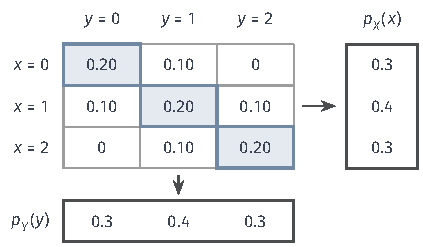
\includegraphics[width=72mm]{figures/07-probability/01-elementary-probability/tikz/rvc-sensor-table/figure.pdf}
  \caption{两台传感器档位的联合概率表。行对应第一台的档位$x$，列对应第二台的档位$y$。浅蓝格子组成事件$\{X=Y\}$；右侧方框是各行之和$p_X(x)$，下方方框是各列之和$p_Y(y)$。}
  \label{fig:rvc-sensor-table}
\end{BookInlineFigure}

由式~\eqref{eq:rvc-joint-pmf-event}，读数一致的概率是对角线三格之和，读数之和至少为$3$的概率是右下角三格之和：
\[
 \mathbb{P}(X=Y)=0.20+0.20+0.20=0.60,
\]
\[
 \mathbb{P}(X+Y\geq 3)=p_{X,Y}(1,2)+p_{X,Y}(2,1)+p_{X,Y}(2,2)=0.40.
\]
两台同时报偏高的概率就是一个格子：$\mathbb{P}(X=2,\,Y=2)=0.20$。这些问题都无法只用每台各自的概率表回答。

\paragraph{联合密度}
如果两个量连续取值，单个点的概率为零，概率表不再适用。一元情形用密度表示单位长度上的质量；平面上相应地用单位面积上的质量。

\begin{definition}[联合密度]
\label{def:rvc-joint-density}
设$f_{X,Y}$是平面上的非负函数。若对每个矩形$R=[a_1,b_1]\times[a_2,b_2]$都有
\begin{equation}
 \mathbb{P}\bigl((X,Y)\in R\bigr)=\iint_{R}f_{X,Y}(x,y)\,\mathrm{d}x\,\mathrm{d}y,
 \label{eq:rvc-joint-density}
\end{equation}
则称$f_{X,Y}$为$(X,Y)$的\term{联合密度}（joint density）。
\end{definition}

矩形概率确定以后，整个联合分布也就确定了：对卷二能够积分的区域$A$，$\mathbb{P}((X,Y)\in A)$同样等于$f_{X,Y}$在$A$上的积分。这一事实的证明需要第~\ref{chap:probability-spaces}章的工具，这里直接使用。多重积分、累次积分以及无界区域上非负函数积分的计算规则，可参考\BookChapterRef{chap:region-integrals}{卷二第24章“区域积分”}。取$A$为整个平面，可知联合密度的积分等于$1$。

联合密度本身不是概率。在点$(x,y)$附近取边长为$h$和$k$的小矩形，若$f_{X,Y}$在该点附近连续，矩形的概率约为$f_{X,Y}(x,y)\,hk$；密度大的地方，同样面积上的概率多。$d$维情形把二重积分换成$d$重积分，把面积换成体积即可。

现在建立贯穿全章的连续例子。令点$(X,Y)$在三角形$T=\{(x,y):0\leq y\leq x\leq 1\}$上均匀分布，即
\begin{equation}
 f_{X,Y}(x,y)=\begin{cases}2,&0\leq y\leq x\leq 1,\\0,&\text{其他}.\end{cases}
 \label{eq:rvc-triangle-density}
\end{equation}
三角形的面积是$1/2$，所以常数取$2$才能使总积分为$1$。“均匀”指同样面积的区域只要都落在三角形内，概率就相同。

求$\mathbb{P}(X+Y\leq 1)$。事件在三角形内对应的部分是顶点为$(0,0)$、$(1,0)$、$(1/2,1/2)$的小三角形，见图~\ref{fig:rvc-triangle-density}(a)。固定$y\in[0,1/2]$，$x$从$y$走到$1-y$，先对$x$积分：
\[
 \mathbb{P}(X+Y\leq 1)=\int_{0}^{1/2}\!\!\int_{y}^{1-y}2\,\mathrm{d}x\,\mathrm{d}y
 =\int_{0}^{1/2}2(1-2y)\,\mathrm{d}y.
\]
再对$y$积分，
\[
 \int_{0}^{1/2}2(1-2y)\,\mathrm{d}y=\Bigl[2y-2y^{2}\Bigr]_{0}^{1/2}=\frac12 .
\]
密度是常数时，概率就是“事件区域面积乘以$2$”：小三角形的面积是$1/4$，结果相同。

\begin{BookInlineFigure}
  \centering
  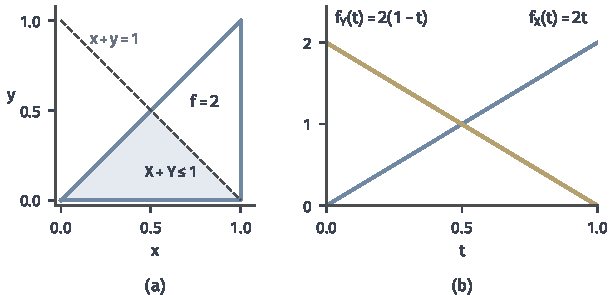
\includegraphics[width=104mm]{figures/07-probability/01-elementary-probability/matplotlib/rvc-triangle-density/figure.pdf}
  \caption{三角形上的均匀密度。(a)蓝线围成的三角形内密度为$2$，其外为$0$；浅蓝区域是事件$\{X+Y\leq 1\}$，概率$1/2$，虚线为$x+y=1$。(b)两个边缘密度：$f_X(t)=2t$（蓝）与$f_Y(t)=2(1-t)$（黄），$t\in[0,1]$。}
  \label{fig:rvc-triangle-density}
\end{BookInlineFigure}

\paragraph{联合分布函数}
概率表只适用于离散情形，联合密度只适用于连续情形。与一元情形一样，分布函数对两类模型都有意义。对$d$维随机向量定义\term{联合分布函数}（joint distribution function）
\begin{equation}
 F_{\bm{X}}(\bm{x})=\mathbb{P}(X_1\leq x_1,\dots,X_d\leq x_d),\qquad \bm{x}\in\mathbb{R}^{d}.
 \label{eq:rvc-joint-cdf}
\end{equation}
二维时，$F_{X,Y}(x,y)$是点$(x,y)$左下方整个象限的概率，见图~\ref{fig:rvc-cdf-rectangle}(a)。

矩形的概率可以由四个角上的分布函数值算出。设$a_1<b_1$，$a_2<b_2$，记$R=(a_1,b_1]\times(a_2,b_2]$。从象限$\{X\leq b_1,Y\leq b_2\}$中去掉$\{X\leq a_1,Y\leq b_2\}$和$\{X\leq b_1,Y\leq a_2\}$，两者的公共部分$\{X\leq a_1,Y\leq a_2\}$被去掉了两次，需要加回一次，于是
\begin{equation}
 \begin{aligned}
 \mathbb{P}\bigl((X,Y)\in R\bigr)
 &=F_{X,Y}(b_1,b_2)-F_{X,Y}(a_1,b_2)\\
 &\quad-F_{X,Y}(b_1,a_2)+F_{X,Y}(a_1,a_2).
 \end{aligned}
 \label{eq:rvc-rectangle}
\end{equation}
图~\ref{fig:rvc-cdf-rectangle}(b)中四个角上的符号就是这四项的正负号。由此可见，分布函数确定全部矩形的概率，从而确定联合分布。

\begin{BookInlineFigure}
  \centering
  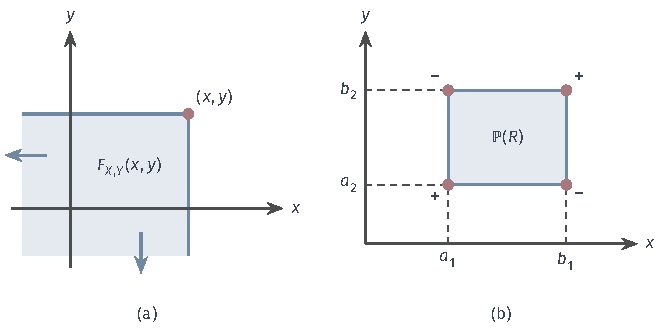
\includegraphics[width=112mm]{figures/07-probability/01-elementary-probability/tikz/rvc-cdf-rectangle/figure.pdf}
  \caption{联合分布函数与矩形概率。(a)$F_{X,Y}(x,y)$是红点左下方象限（浅蓝，向左、向下无界）的概率。(b)矩形$R=(a_1,b_1]\times(a_2,b_2]$的概率等于四个角上分布函数值的带符号和，符号标在各角旁。}
  \label{fig:rvc-cdf-rectangle}
\end{BookInlineFigure}

对三角形模型，$0\leq y\leq x\leq 1$时，左下方象限与三角形的交是梯形$\{(s,t):t\leq s\leq x,\ t\leq y\}$，面积为$xy-y^{2}/2$，乘以密度$2$得
\[
 F_{X,Y}(x,y)=2xy-y^{2},\qquad 0\leq y\leq x\leq 1 .
\]
$0\leq x<y\leq 1$时，象限与三角形的交是$\{t\leq s\leq x\}$，$F_{X,Y}(x,y)=x^{2}$。代入式~\eqref{eq:rvc-rectangle}检验矩形$(1/2,1]\times(0,1/2]$的概率：
\[
 F_{X,Y}(1,\tfrac12)-F_{X,Y}(\tfrac12,\tfrac12)-F_{X,Y}(1,0)+F_{X,Y}(\tfrac12,0)
 =\tfrac34-\tfrac14-0+0=\tfrac12 .
\]
这个正方形整个落在三角形内，面积$1/4$乘以密度$2$也是$1/2$。

\paragraph{边缘分布}
有了联合分布，常常又只关心其中一个分量，例如只问第一台传感器的读数。事件$\{X=x\}$可以按$Y$的取值拆成互斥事件$\{X=x,Y=y\}$的并，由可加性得到
\begin{equation}
 p_X(x)=\sum_{y}p_{X,Y}(x,y),\qquad p_Y(y)=\sum_{x}p_{X,Y}(x,y).
 \label{eq:rvc-marginal-pmf}
\end{equation}
在概率表上，这就是按行求和或按列求和。图~\ref{fig:rvc-sensor-table}中两台传感器的规律相同：
\[
 p_X=p_Y=(0.3,\,0.4,\,0.3).
\]

有联合密度时，取矩形$[a,b]\times[-c,c]$，令$c\to\infty$，先对$y$积分，得到
\[
 \mathbb{P}(a\leq X\leq b)=\int_{a}^{b}\Bigl(\int_{-\infty}^{\infty}f_{X,Y}(x,y)\,\mathrm{d}y\Bigr)\mathrm{d}x .
\]
这里交换顺序与取极限的依据是非负函数的累次积分。上式说明括号里的函数就是$X$的密度：
\begin{equation}
 f_X(x)=\int_{-\infty}^{\infty}f_{X,Y}(x,y)\,\mathrm{d}y,\qquad f_Y(y)=\int_{-\infty}^{\infty}f_{X,Y}(x,y)\,\mathrm{d}x.
 \label{eq:rvc-marginal-density}
\end{equation}
由联合分布得到的单个分量的分布称为\term{边缘分布}（marginal distribution），对其余分量求和或积分的操作称为\term{边缘化}（marginalization）。名称来自概率表：行和与列和写在表的边上。

对三角形模型，固定$x\in[0,1]$，密度只在$0\leq y\leq x$上取$2$；固定$y\in[0,1]$，密度只在$y\leq x\leq 1$上取$2$。于是
\[
 f_X(x)=\int_{0}^{x}2\,\mathrm{d}y=2x,\qquad f_Y(y)=\int_{y}^{1}2\,\mathrm{d}x=2(1-y),
\]
两式都在$[0,1]$上成立，见图~\ref{fig:rvc-triangle-density}(b)。$X$的质量偏向$1$，$Y$的质量偏向$0$：三角形在右侧竖得高，在下方铺得宽。

两颗骰子的例子也可以这样核对。图~\ref{fig:rvc-dice-map}右表中第$m$行有$m-1$个$1$和一个$m$，按行求和得到较大点数的边缘分布
\[
 p_M(m)=\frac{(m-1)+m}{36}=\frac{2m-1}{36},\qquad m=1,\dots,6 .
\]
六个值依次为$1/36,3/36,\dots,11/36$，和为$1$；较大点数偏向大的值。直接从样本空间看，$\{M\leq m\}$要求两颗都不超过$m$，概率为$m^{2}/36$，相邻两项相减同样得到$(2m-1)/36$。

$d$维时规则相同：保留哪些分量，就对其余全部分量求和或积分。例如三维密度$f(x_1,x_2,x_3)$对$x_3$积分得到$(X_1,X_2)$的二维边缘密度，再对$x_2$积分得到$X_1$的边缘密度。用分布函数表示，边缘分布函数是把其余坐标推向$+\infty$的极限，例如$F_X(x)=\lim_{y\to\infty}F_{X,Y}(x,y)$。

\paragraph{相同的边缘，不同的联合}
边缘化把其他分量的信息汇总掉了，这一步一般不能逆转。图~\ref{fig:rvc-same-marginals}把传感器表与另一张表并排放置：右表的每个格子取行和与列和的乘积。两张表的行和、列和完全一样，联合规律却不同。

\begin{BookInlineFigure}
  \centering
  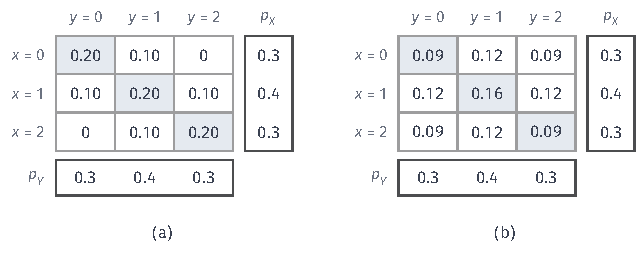
\includegraphics[width=108mm]{figures/07-probability/01-elementary-probability/tikz/rvc-same-marginals/figure.pdf}
  \caption{边缘相同、联合不同的两张概率表。(a)两台传感器的概率表。(b)每格取$p_X(x)p_Y(y)$得到的表。两表的行和与列和都是$(0.3,0.4,0.3)$；浅蓝格子组成事件$\{X=Y\}$，概率分别为$0.60$和$0.34$。}
  \label{fig:rvc-same-marginals}
\end{BookInlineFigure}

右表中读数一致的概率是
\[
 0.09+0.16+0.09=0.34,
\]
远小于左表的$0.60$；右表还允许一台读$0$、另一台读$2$，概率各为$0.09$。只看每台传感器各自的规律，分不出这两种情况。

连续情形也一样。对$\theta\in[-1,1]$，在单位正方形上令
\[
 f_{\theta}(x,y)=1+\theta(1-2x)(1-2y),\qquad 0\leq x,y\leq 1 .
\]
因为$\lvert(1-2x)(1-2y)\rvert\leq 1$，这个函数非负。对$y$积分时，$\int_{0}^{1}(1-2y)\,\mathrm{d}y=0$，所以
\[
 \int_{0}^{1}f_{\theta}(x,y)\,\mathrm{d}y=1+\theta(1-2x)\cdot 0=1 .
\]
同理对$x$积分也得$1$。于是每个$\theta$都给出一个联合密度，两个边缘都是$\operatorname{Unif}(0,1)$。图~\ref{fig:rvc-fgm}中，$\theta=1$时质量偏向两个分量同小或同大的角落，$\theta=-1$时偏向一小一大的角落。

\begin{BookInlineFigure}
  \centering
  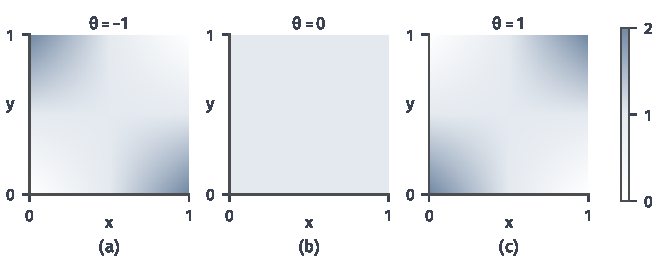
\includegraphics[width=112mm]{figures/07-probability/01-elementary-probability/matplotlib/rvc-fgm/figure.pdf}
  \caption{同样以$\operatorname{Unif}(0,1)$为两个边缘的三个联合密度$f_{\theta}(x,y)=1+\theta(1-2x)(1-2y)$。颜色由白到蓝表示密度由$0$到$2$。(a)$\theta=-1$。(b)$\theta=0$，密度处处为$1$。(c)$\theta=1$。}
  \label{fig:rvc-fgm}
\end{BookInlineFigure}

因此，单独知道每个分量的分布，不足以回答涉及几个分量共同取值的问题。联合分布在边缘之外还记录了分量之间的联系。下一节先研究联系“最弱”的情形：联合分布恰好可以由边缘拼出来。


\section{独立随机变量}
\label{sec:rvc-independence}

图~\ref{fig:rvc-same-marginals}(b)的表是用边缘“乘出来”的。什么时候真实的联合分布恰好就是这张乘积表？第~\ref{chap:classical-probability}章说过，两个事件独立，是指它们同时发生的概率等于各自概率之积。把这一要求加到由两个随机变量生成的每一对事件上，就得到随机变量的独立。

\paragraph{联合分布分解为边缘乘积}
第一台传感器读数落在某个范围，是一个事件；第二台读数落在某个范围，是另一个事件。如果知道其中一个的结果从来不改变另一个的概率，就说两台读数互不提供信息。下面的定义只对区间提出要求，区间可以是单点、有界区间或半直线。

\begin{definition}[独立随机变量]
\label{def:rvc-independence}
若对实数轴上的任意区间$A$和$B$都有
\begin{equation}
 \mathbb{P}(X\in A,\,Y\in B)=\mathbb{P}(X\in A)\,\mathbb{P}(Y\in B),
 \label{eq:rvc-independence}
\end{equation}
则称$X$与$Y$是\term{独立随机变量}（independent random variables），简称$X$与$Y$独立。
\end{definition}

取$A=(-\infty,x]$，$B=(-\infty,y]$，式~\eqref{eq:rvc-independence}给出$F_{X,Y}(x,y)=F_X(x)F_Y(y)$。反过来，若联合分布函数对一切$(x,y)$都分解为边缘分布函数之积，由式~\eqref{eq:rvc-rectangle}，每个半开矩形的概率都分解，独立性的其余情形可由这些矩形取极限得到，这一步留到第~\ref{chap:probability-spaces}章。实际计算中更常用的是下面针对概率表和密度的判别。

\begin{theorem}[独立性的判别]
\label{thm:rvc-independence-criterion}
\begin{enumerate}
 \item 若$X,Y$都只取有限个或可数个值，则$X$与$Y$独立，当且仅当对一切$x,y$，
 \begin{equation}
 p_{X,Y}(x,y)=p_X(x)\,p_Y(y).
 \label{eq:rvc-independence-pmf}
 \end{equation}
 \item 若$(X,Y)$有联合密度，$X,Y$分别有边缘密度$f_X,f_Y$，则$X$与$Y$独立，当且仅当乘积$f_X(x)f_Y(y)$也是$(X,Y)$的联合密度。特别地，若联合密度可以写成$f_{X,Y}(x,y)=g(x)h(y)$，其中$g,h$非负，则$X$与$Y$独立，并且
 \begin{equation}
 f_X=\frac{g}{\int g},\qquad f_Y=\frac{h}{\int h}.
 \label{eq:rvc-factorization}
 \end{equation}
\end{enumerate}
\end{theorem}

\begin{proof}
先看概率表。若$X,Y$独立，取单点区间$A=[x,x]$、$B=[y,y]$，式~\eqref{eq:rvc-independence}就是式~\eqref{eq:rvc-independence-pmf}。反过来，若式~\eqref{eq:rvc-independence-pmf}成立，对任意区间$A,B$，由式~\eqref{eq:rvc-joint-pmf-event}，
\[
 \mathbb{P}(X\in A,\,Y\in B)=\sum_{x\in A}\sum_{y\in B}p_X(x)\,p_Y(y).
\]
各项非负，二重和可以按任意顺序计算，先对$y$求和，得到
\[
 \sum_{x\in A}p_X(x)\sum_{y\in B}p_Y(y)=\mathbb{P}(X\in A)\,\mathbb{P}(Y\in B).
\]

再看密度。若$f_Xf_Y$是联合密度，对矩形$A\times B$，被积函数是$x$的函数与$y$的函数之积，累次积分分开计算：
\[
 \mathbb{P}(X\in A,\,Y\in B)=\int_{A}f_X(x)\,\mathrm{d}x\int_{B}f_Y(y)\,\mathrm{d}y=\mathbb{P}(X\in A)\,\mathbb{P}(Y\in B).
\]
无界区间按非负函数积分取极限理解。反过来，若$X,Y$独立，对每个矩形$R=A\times B$，
\[
 \iint_{R}f_X(x)f_Y(y)\,\mathrm{d}x\,\mathrm{d}y=\mathbb{P}(X\in A)\,\mathbb{P}(Y\in B)=\mathbb{P}\bigl((X,Y)\in R\bigr),
\]
这正是定义~\ref{def:rvc-joint-density}对联合密度的要求。

最后设$f_{X,Y}=gh$。由式~\eqref{eq:rvc-marginal-density}，$f_X(x)=g(x)\int h$，$f_Y(y)=h(y)\int g$；联合密度的总积分为$1$，即$\int g\int h=1$。于是
\[
 f_X(x)f_Y(y)=g(x)h(y)\int g\int h=g(x)h(y)=f_{X,Y}(x,y),
\]
由已证部分，$X$与$Y$独立，式~\eqref{eq:rvc-factorization}也同时得到。
\end{proof}

第二条说“乘积也是联合密度”，而不说“联合密度处处等于乘积”，是因为密度不唯一。把联合密度在一条直线上的值改掉，任何矩形上的积分都不变，改过的函数仍是联合密度，却可能在这条直线上不等于乘积。第~\ref{chap:probability-spaces}章会用“除去面积为零的集合”统一处理这类差别。

\paragraph{判别的例子}
两颗均匀骰子的点数$X_1,X_2$独立：每对点数的概率$1/36$恰好等于$\frac16\cdot\frac16$。同一试验中的$X$与$M$却不独立。由图~\ref{fig:rvc-dice-map}，
\[
 p_{X,M}(2,1)=0,\qquad p_X(2)\,p_M(1)=\frac16\cdot\frac1{36}>0 .
\]
只要找到一个格子不满足式~\eqref{eq:rvc-independence-pmf}，就足以否定独立。

两台传感器也不独立：$p_{X,Y}(0,2)=0$，而$p_X(0)p_Y(2)=0.09$。图~\ref{fig:rvc-same-marginals}(b)那张乘积表描述的才是“边缘相同而相互独立”的两台传感器。对照两张表可以看到，独立是对整张表的要求，九个格子都要分解。

连续情形里，单位正方形上的密度$f(x,y)=4xy$可以写成$(2x)(2y)$，所以两个分量独立，边缘密度都是$2t$，$0\leq t\leq 1$。三角形模型则不独立，理由可以直接从图上读出。取$A=[0,1/2)$，$B=(1/2,1]$，矩形$A\times B$整个落在三角形外，所以$\mathbb{P}(X<1/2,\,Y>1/2)=0$。而由两个边缘密度，
\[
 \mathbb{P}(X<\tfrac12)=\int_{0}^{1/2}2x\,\mathrm{d}x=\tfrac14,\qquad
 \mathbb{P}(Y>\tfrac12)=\int_{1/2}^{1}2(1-y)\,\mathrm{d}y=\tfrac14,
\]
乘积为$1/16\neq 0$。

这个论证给出一条常用的经验：若$X,Y$独立，联合质量只能分布在“$X$可能取的值”与“$Y$可能取的值”组成的乘积形区域上。三角形、圆盘这类不是乘积形的区域上的均匀分布，分量一定不独立。反之，区域是乘积形并不保证独立，图~\ref{fig:rvc-fgm}中$\theta\neq 0$的密度就是反例。

判别定理回答的是“给定联合分布，分量是否独立”。实际建模时常常反过来：两颗骰子分别掷出、两台仪器各自供电，物理上互不影响，于是\emph{假定}它们独立，再用定理~\ref{thm:rvc-independence-criterion}由边缘写出联合分布。这一假定是否合适，要回到试验本身判断；一旦假定错了，例如两台传感器其实受同一股气流影响，按乘积表算出的$\mathbb{P}(X=Y)=0.34$就会低估真实的$0.60$。

\paragraph{多个随机变量的独立}
传感器不止两台时，要求每一组读数范围的联合概率都分解。设$X_1,\dots,X_d$定义在同一样本空间上。若对任意区间$A_1,\dots,A_d$都有
\begin{equation}
 \mathbb{P}(X_1\in A_1,\dots,X_d\in A_d)=\prod_{i=1}^{d}\mathbb{P}(X_i\in A_i),
 \label{eq:rvc-mutual-independence}
\end{equation}
则称$X_1,\dots,X_d$\term{相互独立}（mutually independent）。取某些$A_i$为整个实数轴，这些因子变成$1$，所以任意一部分变量也相互独立。概率表和密度的判别与定理~\ref{thm:rvc-independence-criterion}相同：联合质量函数或联合密度分解为$d$个边缘之积。

只要求每两个变量独立，称为\term{两两独立}（pairwise independent），这比相互独立弱。令$X,Y$独立，各以概率$1/2$取$1$或$-1$，再令$Z=XY$。$(X,Y,Z)$只有四种等可能的取值，即图~\ref{fig:rvc-pairwise}中的四个实心点。

\begin{BookInlineFigure}
  \centering
  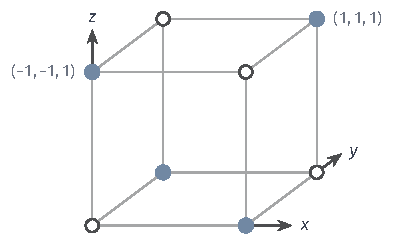
\includegraphics[width=67mm]{figures/07-probability/01-elementary-probability/tikz/rvc-pairwise/figure.pdf}
  \caption{两两独立但不相互独立。$X,Y$是独立的等可能符号，$Z=XY$。立方体八个角中，四个实心点满足$z=xy$，各有概率$1/4$；四个空心点的概率为零。从任一坐标方向把立方体压到一个面上，四个实心点恰好落在该面的四个角，每角$1/4$。}
  \label{fig:rvc-pairwise}
\end{BookInlineFigure}

先验证$X$与$Z$独立。$Z$等可能取$\pm1$。对任意$x,z\in\{1,-1\}$，事件$\{X=x,Z=z\}$就是$\{X=x,Y=xz\}$，于是
\[
 \mathbb{P}(X=x,\,Z=z)=\mathbb{P}(X=x)\,\mathbb{P}(Y=xz)=\tfrac14=\mathbb{P}(X=x)\,\mathbb{P}(Z=z).
\]
同理$Y$与$Z$独立，$X$与$Y$本来独立。三者却不相互独立：
\[
 \mathbb{P}(X=1,\,Y=1,\,Z=-1)=0\neq\tfrac18 .
\]
知道$X$和$Y$以后，$Z$完全确定；而单独知道其中任一个，对$Z$没有任何信息。

\paragraph{独立变量的函数}
传感器读数独立时，把读数换算成温度、取平方或截断，结果仍应独立。下面在概率表的情形证明这一点。设$X,Y$只取有限个或可数个值且独立，$g,h$是实函数。对任意区间$A,B$，令$G=\{x:g(x)\in A\}$，$H=\{y:h(y)\in B\}$，则
\[
 \begin{aligned}
 \mathbb{P}\bigl(g(X)\in A,\,h(Y)\in B\bigr)&=\sum_{x\in G}\sum_{y\in H}p_X(x)\,p_Y(y)\\
 &=\mathbb{P}\bigl(g(X)\in A\bigr)\,\mathbb{P}\bigl(h(Y)\in B\bigr).
 \end{aligned}
\]
所以$g(X)$与$h(Y)$独立。有密度时，集合$G,H$可能不再是区间，同样的结论需要第~\ref{chap:probability-spaces}章对一般集合的处理，这里直接使用。多个变量时结论同样成立：相互独立的变量分成互不相交的几组，各组的函数仍相互独立，例如$X_1+X_2$与$X_3^{2}$独立。

\paragraph{联合分布下的期望}
独立性最常用的推论是乘积的期望可以分开计算。先需要知道怎样对联合分布求期望。第~\ref{chap:random-variable-moments}章对一元情形说明，计算$\mathbb{E}[g(X)]$不必先求$g(X)$的分布。二元情形同样如此：在求和或积分绝对收敛时，
\begin{equation}
 \mathbb{E}\bigl[\varphi(X,Y)\bigr]=\sum_{x,y}\varphi(x,y)\,p_{X,Y}(x,y)
 \quad\text{或}\quad
 \iint\varphi(x,y)\,f_{X,Y}(x,y)\,\mathrm{d}x\,\mathrm{d}y .
 \label{eq:rvc-joint-expectation}
\end{equation}
概率表的情形，把取值对按$\varphi(x,y)$的值分组，同组质量之和就是$\varphi(X,Y)$取该值的概率，于是左右两边是同一个和的两种排列。密度的情形，$\varphi(X,Y)$可能既无概率表也无密度，它的期望及上式的证明要用第~\ref{chap:probability-spaces}章的积分，这里把上式当作计算规则使用。$d$维时把二元和、二重积分换成$d$元和、$d$重积分。

\begin{theorem}[独立变量乘积的期望]
\label{thm:rvc-product-expectation}
设$X$与$Y$独立，$\mathbb{E}\lvert g(X)\rvert<\infty$，$\mathbb{E}\lvert h(Y)\rvert<\infty$。则$g(X)h(Y)$的期望存在，并且
\begin{equation}
 \mathbb{E}\bigl[g(X)h(Y)\bigr]=\mathbb{E}\bigl[g(X)\bigr]\,\mathbb{E}\bigl[h(Y)\bigr].
 \label{eq:rvc-product-expectation}
\end{equation}
\end{theorem}

\begin{proof}
在概率表的情形，由定理~\ref{thm:rvc-independence-criterion}，联合质量等于$p_X(x)p_Y(y)$。先检查绝对收敛：非负项的二重和可以先对$y$求和，
\[
 \sum_{x,y}\lvert g(x)\rvert\,\lvert h(y)\rvert\,p_X(x)\,p_Y(y)
 =\Bigl(\sum_{x}\lvert g(x)\rvert p_X(x)\Bigr)\Bigl(\sum_{y}\lvert h(y)\rvert p_Y(y)\Bigr)<\infty .
\]
因此由式~\eqref{eq:rvc-joint-expectation}，$\mathbb{E}[g(X)h(Y)]$存在。绝对收敛的二重和同样可以先对$y$求和，去掉绝对值重复上面的计算，就得到式~\eqref{eq:rvc-product-expectation}。在密度的情形，取$f_Xf_Y$为联合密度，把求和换成积分：先对非负的$\lvert g(x)h(y)\rvert f_X(x)f_Y(y)$做累次积分，确认积分有限，再按绝对可积函数的累次积分规则分开计算。
\end{proof}

可积条件的作用是保证求和与积分的次序可以交换；只有两个期望都有限，右边的乘积才有意义。例如两颗骰子的点数之积，期望为$(7/2)^{2}=49/4$；$f=4xy$的模型中，
\[
 \mathbb{E}[XY]=\int_{0}^{1}\!\!\int_{0}^{1}xy\cdot 4xy\,\mathrm{d}x\,\mathrm{d}y=4\cdot\frac13\cdot\frac13=\frac49 ,
\]
恰好是$\mathbb{E}[X]^{2}=(2/3)^{2}$。

定理也可以反过来用于否定独立。三角形模型中$\mathbb{E}[X]=2/3$，$\mathbb{E}[Y]=1/3$，而
\[
 \mathbb{E}[XY]=\int_{0}^{1}\!\!\int_{0}^{x}2xy\,\mathrm{d}y\,\mathrm{d}x=\int_{0}^{1}x^{3}\,\mathrm{d}x=\frac14\neq\frac29 .
\]
但等式~\eqref{eq:rvc-product-expectation}只对一对特定的函数成立时，并不能推出独立，第~\ref{sec:rvc-moments}节会给出反例。

\paragraph{独立同分布}
重复试验的标准模型是：每次试验在相同条件下进行，各次结果互不影响。用随机变量写出来，就是下面的两个要求同时成立。若$X_1,\dots,X_n$相互独立，并且具有同一个分布$P$，则称它们\term{独立同分布}（independent and identically distributed），简记为i.i.d.，并写
\begin{equation}
 X_1,\dots,X_n\overset{\text{i.i.d.}}{\sim}P .
 \label{eq:rvc-iid}
\end{equation}
由定理~\ref{thm:rvc-independence-criterion}，它们的联合质量函数或联合密度是同一个边缘的$n$次乘积，例如$\prod_{i=1}^{n}p(x_i)$。

“同分布”只约束每个分量各自的规律，“独立”只约束分量之间的关系，两者谁也推不出谁。图~\ref{fig:rvc-iid}用两颗骰子说明三种情况。(a)两颗骰子独立掷出，$36$个格点各有$1/36$，两项都满足。(b)令$X_2=X_1$，两个分量同分布，但质量全在对角线上，不独立。(c)$X_1$是骰子点数，$X_2$是独立抛出的均匀硬币，记正面为$1$，两者独立但分布不同。

\begin{BookInlineFigure}
  \centering
  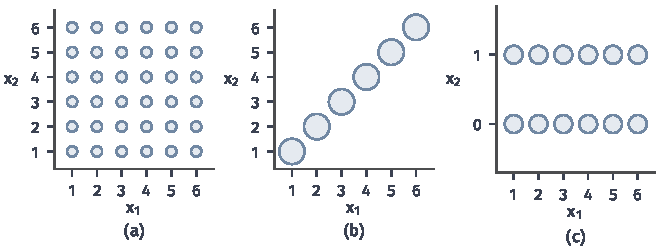
\includegraphics[width=112mm]{figures/07-probability/01-elementary-probability/matplotlib/rvc-iid/figure.pdf}
  \caption{独立与同分布是两项不同的要求，圆的面积正比于联合质量。(a)两颗独立的均匀骰子，每点$1/36$。(b)$X_2=X_1$，对角线上每点$1/6$：同分布，不独立。(c)骰子点数$X_1$与独立的均匀硬币$X_2\in\{0,1\}$，每点$1/12$：独立，不同分布。}
  \label{fig:rvc-iid}
\end{BookInlineFigure}

在(b)中，两次“试验”其实只做了一次，第二个数只是抄写第一个；在(c)中，两次试验互不影响，但做的不是同一种试验。只有(a)对应“同一试验独立重复两次”。后面讨论样本平均为什么随次数增加而稳定时，两项要求分别承担不同作用：同分布保证每次平均的是同一个量，独立保证波动能互相抵消，见第~\ref{chap:laws-of-large-numbers}章。


\section{均值与协方差}
\label{sec:rvc-moments}

把两台传感器的读数取平均，波动能减小多少？若两台独立，直觉告诉我们方差减半；可是图~\ref{fig:rvc-sensor-table}的两台读数倾向于一致，平均以后的改善应当少一些。要把“少多少”算出来，需要一个能概括两个量一起偏离中心的数。完整的联合分布在高维时难以列出，这一节用均值向量和协方差矩阵概括它的中心与波动。全节假定所涉及的各分量都有有限二阶矩，即$\mathbb{E}[X_i^{2}]<\infty$；只用到均值的地方，有限一阶矩就够了。

\paragraph{均值向量}
随机向量的中心可以逐个分量描述。设每个分量都有有限期望，定义\term{均值向量}（mean vector）
\begin{equation}
 \bm{\mu}=\mathbb{E}[\bm{X}]=\bigl(\mathbb{E}[X_1],\dots,\mathbb{E}[X_d]\bigr)^{\top}.
 \label{eq:rvc-mean-vector}
\end{equation}
一元时期望是质量分布的重心；这里$\bm{\mu}$是平面或空间中质量分布的重心。传感器表中$\bm{\mu}=(1,1)^{\top}$。三角形模型中，由边缘密度，
\[
 \mathbb{E}[X]=\int_{0}^{1}x\cdot 2x\,\mathrm{d}x=\frac23,\qquad \mathbb{E}[Y]=\int_{0}^{1}y\cdot 2(1-y)\,\mathrm{d}y=\frac13,
\]
$\bm{\mu}=(2/3,1/3)^{\top}$，正是三角形三个顶点坐标的平均，也就是均匀薄板的重心。

期望对随机向量是线性的。在式~\eqref{eq:rvc-joint-expectation}中取$\varphi(x,y)=x+y$，把和或积分拆成两项，得到$\mathbb{E}[X+Y]=\mathbb{E}[X]+\mathbb{E}[Y]$。逐行使用这一点，对$m\times d$常矩阵$\bm{A}$和常向量$\bm{b}\in\mathbb{R}^{m}$，
\begin{equation}
 \mathbb{E}[\bm{A}\bm{X}+\bm{b}]=\bm{A}\bm{\mu}+\bm{b}.
 \label{eq:rvc-mean-affine}
\end{equation}
这里不需要分量之间有任何独立性。矩阵按全书约定用粗体大写字母表示，后面的协方差矩阵$\bm{\Sigma}$也是如此。

\paragraph{协方差与交叉项}
和的均值只依赖各分量的均值，和的方差却不同。记$\mu_X=\mathbb{E}[X]$，$\mu_Y=\mathbb{E}[Y]$，把$X+Y$减去均值后平方展开：
\[
 \operatorname{Var}(X+Y)=\mathbb{E}\Bigl[\bigl((X-\mu_X)+(Y-\mu_Y)\bigr)^{2}\Bigr].
\]
平方展开成三项，再由期望的线性，
\[
 \operatorname{Var}(X+Y)=\operatorname{Var}(X)+\operatorname{Var}(Y)+2\,\mathbb{E}\bigl[(X-\mu_X)(Y-\mu_Y)\bigr].
\]
前两项只依赖边缘分布，最后一项依赖联合分布。这个交叉项就是我们要找的量。

\begin{definition}[协方差]
\label{def:rvc-covariance}
设$\mathbb{E}[X^{2}]<\infty$，$\mathbb{E}[Y^{2}]<\infty$。称
\begin{equation}
 \operatorname{Cov}(X,Y)=\mathbb{E}\bigl[(X-\mu_X)(Y-\mu_Y)\bigr]
 \label{eq:rvc-covariance}
\end{equation}
为$X$与$Y$的\term{协方差}（covariance）。
\end{definition}

有限二阶矩保证这个期望存在：由$\lvert uv\rvert\leq(u^{2}+v^{2})/2$，中心化乘积的绝对值被两个平方项之和控制。展开乘积并用线性，得到常用的计算公式
\begin{equation}
 \operatorname{Cov}(X,Y)=\mathbb{E}[XY]-\mu_X\mu_Y .
 \label{eq:rvc-covariance-formula}
\end{equation}

中心化乘积$(X-\mu_X)(Y-\mu_Y)$的符号有直观意义。以均值点$(\mu_X,\mu_Y)$为原点把平面分成四个象限：两个量同时偏高或同时偏低时，乘积为正；一高一低时，乘积为负。协方差把每个取值对的乘积按质量加权求和。为正，说明“同向偏离”的质量占优；为负，说明“反向偏离”占优。

图~\ref{fig:rvc-cov-quadrants}把传感器表的九个格子画成圆，并标出每格对协方差的贡献$(x-1)(y-1)p_{X,Y}(x,y)$。位于均值线上的格子贡献为零；四个角中，左下与右上各贡献$+0.20$，另两角的概率为零。于是
\[
 \operatorname{Cov}(X,Y)=0.20+0.20=0.40 .
\]
用式~\eqref{eq:rvc-covariance-formula}核对：$XY$只在$x,y\geq1$的四格非零，
\[
 \mathbb{E}[XY]=1\cdot0.20+2\cdot0.10+2\cdot0.10+4\cdot0.20=1.4,
\]
\[
 \operatorname{Cov}(X,Y)=1.4-1\cdot1=0.4 .
\]

\begin{BookInlineFigure}
  \centering
  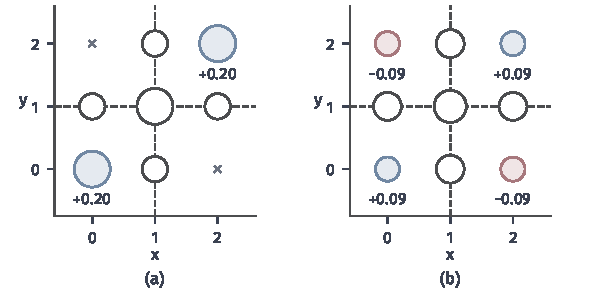
\includegraphics[width=100mm]{figures/07-probability/01-elementary-probability/matplotlib/rvc-cov-quadrants/figure.pdf}
  \caption{协方差是中心化乘积的加权和。圆的面积正比于格子的概率，虚线过均值$(1,1)$。蓝色格子的贡献$(x-1)(y-1)p_{X,Y}(x,y)$为正，红色为负，白色为零，叉号表示概率为零的格子；数字是各格的贡献。(a)传感器表，协方差$0.40$。(b)边缘相同的乘积表，正负贡献抵消，协方差为$0$。}
  \label{fig:rvc-cov-quadrants}
\end{BookInlineFigure}

协方差关于每个变量都是线性的，并且不受平移影响。由定义直接得到：对常数$a,b,c,e$，
\[
 \operatorname{Cov}(aX+b,\,cY+e)=ac\operatorname{Cov}(X,Y),\qquad \operatorname{Cov}(X,X)=\operatorname{Var}(X),
\]
并且对第三个二阶矩有限的变量$X_2$，
\[
 \operatorname{Cov}(X+X_2,\,Y)=\operatorname{Cov}(X,Y)+\operatorname{Cov}(X_2,Y).
\]把这些性质用于$\sum_i a_iX_i$与它自己，就得到有限和的方差展开：
\begin{equation}
 \operatorname{Var}\Bigl(\sum_{i=1}^{n}a_iX_i\Bigr)=\sum_{i=1}^{n}a_i^{2}\operatorname{Var}(X_i)+2\sum_{i<j}a_ia_j\operatorname{Cov}(X_i,X_j).
 \label{eq:rvc-variance-sum}
\end{equation}
$n$个对角项来自各分量自身的波动，$n(n-1)/2$个交叉项来自两两之间的共同波动。

用传感器表算一算。由式~\eqref{eq:rvc-variance-sum}，
\[
 \operatorname{Var}(X+Y)=0.6+0.6+2\cdot0.4=2.0 .
\]
直接核对：把表中格子按$x+y$的值分组，$X+Y$在$\{0,1,2,3,4\}$上各取概率$0.2$，均值为$2$，方差为$(4+1+0+1+4)\times0.2=2$。两台读数的平均$(X+Y)/2$方差为$2.0/4=0.5$，只比单台的$0.6$小一点；若换成图~\ref{fig:rvc-same-marginals}(b)那样独立的两台，交叉项为零，平均的方差是$1.2/4=0.3$，正好减半。

交叉项的符号随系数而变。两台读数之差的方差是
\[
 \operatorname{Var}(X-Y)=0.6+0.6-2\cdot0.4=0.4 .
\]
直接核对：$X-Y$以概率$0.6$取$0$，以概率$0.2$各取$\pm1$，方差为$0.4$。正相关使和的波动变大、差的波动变小，所以比较两台读数之差，比单看一台更容易发现某台失灵：正常时差几乎总在$0$附近。

\paragraph{协方差矩阵}
$d$个分量两两之间都有协方差，排成矩阵便于统一计算。定义\term{协方差矩阵}（covariance matrix）
\begin{equation}
 \bm{\Sigma}=\operatorname{Cov}(\bm{X})=\mathbb{E}\bigl[(\bm{X}-\bm{\mu})(\bm{X}-\bm{\mu})^{\top}\bigr],\qquad
 \bm{\Sigma}_{i,j}=\operatorname{Cov}(X_i,X_j),
 \label{eq:rvc-covariance-matrix}
\end{equation}
其中矩阵的期望逐个元素计算。对角元是各分量的方差，非对角元是协方差。传感器表和三角形模型的协方差矩阵分别是
\[
 \begin{bmatrix}0.6&0.4\\0.4&0.6\end{bmatrix},\qquad
 \begin{bmatrix}1/18&1/36\\1/36&1/18\end{bmatrix}.
\]
后者由边缘密度算出$\mathbb{E}[X^{2}]=1/2$、$\mathbb{E}[Y^{2}]=1/6$，再用上一节的$\mathbb{E}[XY]=1/4$：
\[
 \operatorname{Var}(X)=\tfrac12-\tfrac49=\tfrac1{18},\quad
 \operatorname{Var}(Y)=\tfrac16-\tfrac19=\tfrac1{18},\quad
 \operatorname{Cov}(X,Y)=\tfrac14-\tfrac29=\tfrac1{36}.
\]

式~\eqref{eq:rvc-variance-sum}写成矩阵形式，就是协方差矩阵最重要的性质。

\begin{theorem}[协方差矩阵的性质]
\label{thm:rvc-covariance-matrix}
设$\bm{X}$的各分量有有限二阶矩，协方差矩阵为$\bm{\Sigma}$。对常向量$\bm{a},\bm{b}\in\mathbb{R}^{d}$，
\begin{equation}
 \operatorname{Cov}(\bm{a}^{\top}\bm{X},\,\bm{b}^{\top}\bm{X})=\bm{a}^{\top}\bm{\Sigma}\bm{b},\qquad
 \operatorname{Var}(\bm{a}^{\top}\bm{X})=\bm{a}^{\top}\bm{\Sigma}\bm{a}\geq 0 .
 \label{eq:rvc-quadratic-form}
\end{equation}
因此$\bm{\Sigma}$对称半正定。对$m\times d$常矩阵$\bm{A}$和常向量$\bm{b}\in\mathbb{R}^{m}$，
\begin{equation}
 \operatorname{Cov}(\bm{A}\bm{X}+\bm{b})=\bm{A}\bm{\Sigma}\bm{A}^{\top}.
 \label{eq:rvc-covariance-affine}
\end{equation}
\end{theorem}

\begin{proof}
协方差的定义关于两个变量对称，所以$\bm{\Sigma}$对称。由式~\eqref{eq:rvc-mean-affine}，$\bm{a}^{\top}\bm{X}$的均值是$\bm{a}^{\top}\bm{\mu}$，所以它的中心化是$\bm{a}^{\top}(\bm{X}-\bm{\mu})$；$\bm{b}^{\top}\bm{X}$同理。两个标量之积可以写成
\[
 \bigl(\bm{a}^{\top}(\bm{X}-\bm{\mu})\bigr)\bigl(\bm{b}^{\top}(\bm{X}-\bm{\mu})\bigr)
 =\bm{a}^{\top}(\bm{X}-\bm{\mu})(\bm{X}-\bm{\mu})^{\top}\bm{b}.
\]
右边是矩阵元素的线性组合，取期望时可以逐项进行，得到$\bm{a}^{\top}\bm{\Sigma}\bm{b}$。取$\bm{b}=\bm{a}$，左边是方差，必不小于零，这对一切$\bm{a}$成立，所以$\bm{\Sigma}$半正定。最后，$\bm{A}\bm{X}+\bm{b}$的第$i$个分量是$\bm{A}_{i,:}\bm{X}+b_i$，常数不影响协方差，由第一式，它与第$j$个分量的协方差为$\bm{A}_{i,:}\bm{\Sigma}\bm{A}_{j,:}^{\top}$，这正是$\bm{A}\bm{\Sigma}\bm{A}^{\top}$的$(i,j)$元。
\end{proof}

用式~\eqref{eq:rvc-covariance-affine}可以一次算出几个线性组合的全部方差与协方差。对传感器读数取平均$Z=(X+Y)/2$与差$W=X-Y$，即
\[
 \begin{bmatrix}Z\\W\end{bmatrix}=\bm{A}\begin{bmatrix}X\\Y\end{bmatrix},\qquad
 \bm{A}=\begin{bmatrix}1/2&1/2\\1&-1\end{bmatrix}.
\]
矩阵相乘得到
\[
 \bm{A}\bm{\Sigma}\bm{A}^{\top}
 =\begin{bmatrix}1/2&1/2\\1&-1\end{bmatrix}\begin{bmatrix}0.6&0.4\\0.4&0.6\end{bmatrix}\begin{bmatrix}1/2&1\\1/2&-1\end{bmatrix}
 =\begin{bmatrix}0.5&0\\0&0.4\end{bmatrix}.
\]
对角元与前面分别算出的$0.5$、$0.4$一致；非对角元为零，说明平均与差不相关。原因是两台读数方差相等：由协方差的双线性，交叉的两项互相抵消，
\[
 \operatorname{Cov}(Z,W)=\tfrac12\bigl(\operatorname{Var}(X)-\operatorname{Var}(Y)\bigr)=0 .
\]不相关并不等于独立，例如$W=\pm1$时$Z$只能取$1/2$或$3/2$，而$W=0$时$Z$可以取$0,1,2$。

式~\eqref{eq:rvc-quadratic-form}给协方差矩阵一个几何解释。取单位向量$\bm{a}$，$\bm{a}^{\top}(\bm{X}-\bm{\mu})$是点$\bm{X}$在方向$\bm{a}$上相对重心的有向距离，所以$\bm{a}^{\top}\bm{\Sigma}\bm{a}$是质量沿方向$\bm{a}$的散开程度。把概率看作质量，这正是力学中薄板绕“过重心且垂直于$\bm{a}$的直线”的转动惯量；一元方差是它的一维特例。

$\bm{\Sigma}$是实对称矩阵，可以正交对角化，单位特征向量给出散开程度最大和最小的方向，对应的特征值就是沿这些方向的方差，可参考\BookChapterRef{chap:eigen-spectral-decomposition}{卷二第6章“谱分解”}。三角形模型中，取$\bm{a}=(\cos\varphi,\sin\varphi)^{\top}$，
\[
 v(\varphi)=\bm{a}^{\top}\bm{\Sigma}\bm{a}=\frac{1}{18}+\frac{\sin 2\varphi}{36}.
\]
$\varphi=\pi/4$时取最大值$1/12$，方向$(1,1)^{\top}/\sqrt2$；$\varphi=3\pi/4$时取最小值$1/36$，方向$(1,-1)^{\top}/\sqrt2$。两者正是$\bm{\Sigma}$的两个特征值和特征向量，见图~\ref{fig:rvc-cov-ellipse}。

\begin{BookInlineFigure}
  \centering
  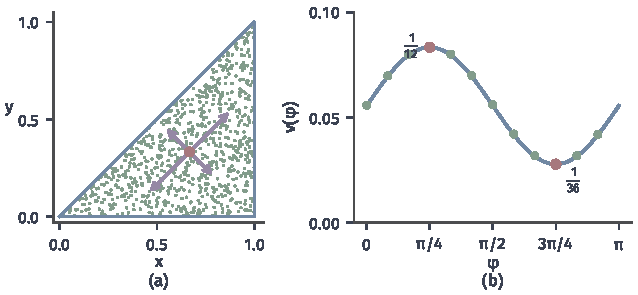
\includegraphics[width=108mm]{figures/07-probability/01-elementary-probability/matplotlib/rvc-cov-ellipse/figure.pdf}
  \caption{协方差矩阵与散开方向。(a)三角形模型的$800$个模拟点（绿，种子$1$），红点为均值$(2/3,1/3)$，紫色双箭头沿两个特征向量，半长等于该方向的标准差$\sqrt{1/12}$与$\sqrt{1/36}$。(b)方向$(\cos\varphi,\sin\varphi)$上的方差$v(\varphi)$（蓝线），红点为最大值与最小值，绿点是同一批模拟点投影后的样本方差。}
  \label{fig:rvc-cov-ellipse}
\end{BookInlineFigure}

半正定而不正定时，存在非零$\bm{a}$使$\bm{a}^{\top}\bm{\Sigma}\bm{a}=0$。这时$\bm{a}^{\top}\bm{X}$的方差为零，由第~\ref{chap:tail-probabilities}章的Chebyshev不等式，对每个$\varepsilon>0$，
\[
 \mathbb{P}\bigl(\lvert\bm{a}^{\top}\bm{X}-\bm{a}^{\top}\bm{\mu}\rvert\geq\varepsilon\bigr)\leq\frac{0}{\varepsilon^{2}}=0 .
\]
也就是说，$\bm{X}$偏离超平面$\bm{a}^{\top}\bm{x}=\bm{a}^{\top}\bm{\mu}$任何正距离的概率都是零，质量全部压在这个超平面上。例如把传感器读数排成$\bm{X}=(X,Y,X+Y)^{\top}$，由式~\eqref{eq:rvc-covariance-affine}，
\[
 \bm{\Sigma}=\begin{bmatrix}0.6&0.4&1.0\\0.4&0.6&1.0\\1.0&1.0&2.0\end{bmatrix},\qquad
 \bm{\Sigma}\begin{bmatrix}1\\1\\-1\end{bmatrix}=\bm{0}.
\]
零特征值对应的方向$(1,1,-1)^{\top}$正好表达了第三个分量等于前两个之和。这种由线性约束造成的奇异协方差，在第~\ref{chap:multivariate-distributions}章的计数向量中还会遇到。

\paragraph{相关系数}
协方差的数值依赖单位：把温度从摄氏度换成另一种刻度，乘以常数$c$，协方差也乘以$c$，而两台传感器之间的联系并没有改变。除以两个标准差，就得到与单位无关的量。

\begin{definition}[相关系数]
\label{def:rvc-correlation}
设$0<\operatorname{Var}(X)<\infty$，$0<\operatorname{Var}(Y)<\infty$，记$\sigma_X,\sigma_Y$为标准差。称
\begin{equation}
 \rho_{X,Y}=\frac{\operatorname{Cov}(X,Y)}{\sigma_X\sigma_Y}
 \label{eq:rvc-correlation}
\end{equation}
为$X$与$Y$的\term{相关系数}（correlation coefficient），不致混淆时简写为$\rho$。
\end{definition}

\begin{theorem}[相关系数的范围]
\label{thm:rvc-correlation-bound}
在上述条件下$-1\leq\rho_{X,Y}\leq 1$。若$\rho_{X,Y}=\pm1$，记
\begin{equation}
 L=\mu_Y+\rho_{X,Y}\frac{\sigma_Y}{\sigma_X}(X-\mu_X),
 \label{eq:rvc-correlation-line}
\end{equation}
则对每个$\varepsilon>0$有$\mathbb{P}(\lvert Y-L\rvert\geq\varepsilon)=0$。反过来，若$Y=a+bX$，$b\neq0$，则$\rho_{X,Y}$等于$b$的符号。
\end{theorem}

\begin{proof}
把两个变量标准化，令$U=(X-\mu_X)/\sigma_X$，$V=(Y-\mu_Y)/\sigma_Y$，则
\[
 \mathbb{E}[U^{2}]=\mathbb{E}[V^{2}]=1,\qquad \mathbb{E}[UV]=\rho .
\]
考虑非负随机变量$(V-\rho U)^{2}$，展开后取期望：
\[
 0\leq\mathbb{E}\bigl[(V-\rho U)^{2}\bigr]=\mathbb{E}[V^{2}]-2\rho\,\mathbb{E}[UV]+\rho^{2}\mathbb{E}[U^{2}]=1-\rho^{2},
\]
所以$\rho^{2}\leq1$。

若$\rho^{2}=1$，上式说明$\mathbb{E}[(V-\rho U)^{2}]=0$。对每个$\delta>0$，由第~\ref{chap:tail-probabilities}章的Markov不等式，
\[
 \mathbb{P}\bigl(\lvert V-\rho U\rvert\geq\delta\bigr)=\mathbb{P}\bigl((V-\rho U)^{2}\geq\delta^{2}\bigr)\leq\frac{0}{\delta^{2}}=0 .
\]
由式~\eqref{eq:rvc-correlation-line}，$\sigma_Y(V-\rho U)=Y-L$，取$\delta=\varepsilon/\sigma_Y$即得结论。

反过来，若$Y=a+bX$，则$\operatorname{Cov}(X,Y)=b\sigma_X^{2}$，$\sigma_Y=\lvert b\rvert\sigma_X$，代入式~\eqref{eq:rvc-correlation}得$\rho=b/\lvert b\rvert$。
\end{proof}

这个证明与内积空间中的Cauchy--Schwarz不等式是同一个论证：把$\mathbb{E}[UV]$看作两个中心化变量的内积，相关系数就是它们夹角的余弦，可参考\BookChapterRef{chap:inner-product-spaces}{卷二第4章“内积空间”}。定理的第二部分只说$Y$偏离直线$L$任何正距离的概率为零；第~\ref{chap:probability-spaces}章会说明这等价于$\mathbb{P}(Y=L)=1$。

两个贯穿例子的相关系数是
\[
 \rho_{\text{传感器}}=\frac{0.4}{\sqrt{0.6\cdot0.6}}=\frac23,\qquad
 \rho_{\text{三角形}}=\frac{1/36}{\sqrt{(1/18)(1/18)}}=\frac12 .
\]
对图~\ref{fig:rvc-fgm}的密度族，两个边缘的均值都是$1/2$，密度中的常数项$1$对应独立部分，贡献的协方差为零，于是
\[
 \operatorname{Cov}(X,Y)=\theta\Bigl(\int_{0}^{1}x(1-2x)\,\mathrm{d}x\Bigr)^{2}=\theta\Bigl(-\frac16\Bigr)^{2}=\frac{\theta}{36}.
\]
边缘方差为$1/12$，所以$\rho=\theta/3$，绝对值不超过$1/3$：这个族只能表达较弱的联系。

相关系数衡量的是散点向一条直线集中的程度，而不是直线的斜率。图~\ref{fig:rvc-correlation}前三幅中，$\rho=0.9$的点紧贴上升直线，$\rho=-0.6$的点较松散地沿下降方向分布，$\rho=0$的点看不出线性趋势。第四幅中$Y$几乎由$X$决定，相关系数却为零：抛物线左右两支对“同向”和“反向”的贡献互相抵消。

\begin{BookInlineFigure}
  \centering
  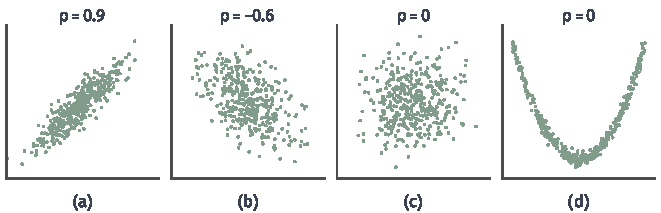
\includegraphics[width=112mm]{figures/07-probability/01-elementary-probability/matplotlib/rvc-correlation/figure.pdf}
  \caption{不同相关系数下的散点，每幅$400$个模拟点（种子$7$）。(a)至(c)中$X,Y$都服从$\mathcal{N}(0,1)$，取$Y=\rho X+\sqrt{1-\rho^{2}}\,Z$，$Z\sim\mathcal{N}(0,1)$与$X$独立，相关系数分别为$0.9$、$-0.6$、$0$。(d)中$X\sim\operatorname{Unif}(-\sqrt3,\sqrt3)$，$Y=X^{2}-1+0.1Z$，相关系数为$0$。}
  \label{fig:rvc-correlation}
\end{BookInlineFigure}

“集中于直线的程度”可以精确表述。用直线$a+bX$近似$Y$，以均方误差$\mathbb{E}[(Y-a-bX)^{2}]$衡量好坏。对固定的$b$，记$W=Y-bX$。把$W-a$拆成$(W-\mathbb{E}[W])+(\mathbb{E}[W]-a)$，交叉项的期望为零，于是
\[
 \mathbb{E}\bigl[(W-a)^{2}\bigr]=\operatorname{Var}(W)+\bigl(\mathbb{E}[W]-a\bigr)^{2}.
\]
最好的$a$是$\mathbb{E}[W]$，剩下的误差是
\[
 \operatorname{Var}(Y-bX)=\operatorname{Var}(Y)-2b\operatorname{Cov}(X,Y)+b^{2}\operatorname{Var}(X).
\]
这是$b$的二次函数，对$b$求导并令导数为零，最小点是
\[
 b^{*}=\frac{\operatorname{Cov}(X,Y)}{\operatorname{Var}(X)}.
\]
代回得到最小均方误差
\begin{equation}
 \min_{a,b}\mathbb{E}\bigl[(Y-a-bX)^{2}\bigr]=\operatorname{Var}(Y)\,(1-\rho_{X,Y}^{2}).
 \label{eq:rvc-best-line}
\end{equation}
所以$\rho^{2}$是最佳直线能解释的那一部分方差。$\rho=0$时最佳斜率为零，直线对预测$Y$毫无帮助；但这只说明直线无用，曲线仍可能很有用，图~\ref{fig:rvc-correlation}(d)就是这样。

\paragraph{平均能把波动降低多少}
现在回答本节开头的问题。设$n$台传感器的读数$X_1,\dots,X_n$方差都是$\sigma^{2}$，任意两台的相关系数都是$\rho$，即协方差都是$\rho\sigma^{2}$。由式~\eqref{eq:rvc-variance-sum}，取$a_i=1/n$，对角项共$n$个，交叉项共$n(n-1)/2$个，
\[
 \operatorname{Var}(\bar{X}_n)=\frac{1}{n^{2}}\Bigl(n\sigma^{2}+n(n-1)\rho\sigma^{2}\Bigr),
\]
其中$\bar{X}_n=(X_1+\dots+X_n)/n$。整理得
\begin{equation}
 \operatorname{Var}(\bar{X}_n)=\sigma^{2}\Bigl(\frac1n+\Bigl(1-\frac1n\Bigr)\rho\Bigr).
 \label{eq:rvc-equicorrelated-average}
\end{equation}

两台传感器的情形，$n=2$，$\sigma^{2}=0.6$，$\rho=2/3$，代入得$0.6\times(1/2+1/3)=0.5$，与前面直接计算的结果一致。$\rho=0$时上式变成$\sigma^{2}/n$，平均$n$次把方差降为$1/n$。$\rho>0$时，$n\to\infty$，方差趋于$\rho\sigma^{2}$而不是零：各台共有的那部分波动，例如同一股气流同时影响所有传感器，无论平均多少台都消不掉。

\begin{BookInlineFigure}
  \centering
  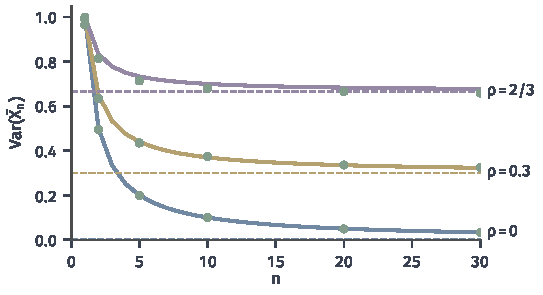
\includegraphics[width=92mm]{figures/07-probability/01-elementary-probability/matplotlib/rvc-average-variance/figure.pdf}
  \caption{$n$个方差为$1$、两两相关系数为$\rho$的读数，其平均的方差。实线是式~\eqref{eq:rvc-equicorrelated-average}，蓝、黄、紫分别对应$\rho=0,0.3,2/3$；虚线是极限$\rho$。绿点是$4000$次模拟的样本方差（种子$11$），每次取$X_i=\sqrt{\rho}\,Z_0+\sqrt{1-\rho}\,Z_i$，$Z_0,Z_1,\dots$相互独立且服从$\mathcal{N}(0,1)$。}
  \label{fig:rvc-average-variance}
\end{BookInlineFigure}

图~\ref{fig:rvc-average-variance}中，模拟用的构造$X_i=\sqrt{\rho}\,Z_0+\sqrt{1-\rho}\,Z_i$把每个读数拆成共同部分$Z_0$和各自部分$Z_i$。平均时各自部分的方差按$1/n$缩小，共同部分原样保留，这正是式~\eqref{eq:rvc-equicorrelated-average}两项的来源。

\paragraph{相关与独立}
协方差为零的两个变量称为\term{不相关}（uncorrelated）。独立变量一定不相关：若$X,Y$独立且二阶矩有限，在定理~\ref{thm:rvc-product-expectation}中取$g(x)=x-\mu_X$，$h(y)=y-\mu_Y$，得到
\[
 \operatorname{Cov}(X,Y)=\mathbb{E}[X-\mu_X]\,\mathbb{E}[Y-\mu_Y]=0 .
\]
因此两两独立的变量之和，方差等于方差之和；式~\eqref{eq:rvc-variance-sum}只需要交叉项为零，也就是只需要两两不相关。

反过来不成立，因为协方差只检查一种特定的乘积。令$X$等可能取$-1,0,1$，$Y=X^{2}$。则$\mathbb{E}[X]=0$，$\mathbb{E}[XY]=\mathbb{E}[X^{3}]=0$，所以$\operatorname{Cov}(X,Y)=0$。可是$Y$完全由$X$决定，独立性不成立：
\[
 \mathbb{P}(X=0,\,Y=1)=0\neq\mathbb{P}(X=0)\,\mathbb{P}(Y=1)=\tfrac13\cdot\tfrac23 .
\]

连续的例子是单位圆盘上的均匀分布，密度在圆盘内为$1/\pi$。把$(x,y)$换成$(-x,y)$，密度不变而$xy$变号，所以$\mathbb{E}[XY]=-\mathbb{E}[XY]=0$；同理$\mathbb{E}[X]=0$，协方差为零。圆盘不是乘积形区域，按上一节的判别，两个分量不独立。具体地，$\mathbb{P}(X>0.9)$与$\mathbb{P}(Y>0.5)$都为正，而点$(x,y)$满足$x>0.9$、$y>0.5$时$x^{2}+y^{2}>0.81+0.25>1$，落在圆盘外，所以$\mathbb{P}(X>0.9,\,Y>0.5)=0$。

\begin{BookInlineFigure}
  \centering
  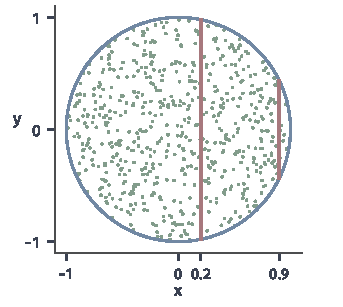
\includegraphics[width=58mm]{figures/07-probability/01-elementary-probability/matplotlib/rvc-disk/figure.pdf}
  \caption{单位圆盘上的均匀分布：不相关但不独立。绿点是$600$个模拟点（种子$3$），样本相关系数约为$-0.01$。红线段是$x=0.2$与$x=0.9$处$y$能取到的范围，分别为$\lvert y\rvert\leq0.98$和$\lvert y\rvert\leq0.44$。}
  \label{fig:rvc-disk}
\end{BookInlineFigure}

图~\ref{fig:rvc-disk}显示了依赖的方式：$X$靠近$\pm1$时，$Y$被挤到$0$附近，$X$靠近$0$时，$Y$可以取到$\pm1$附近。依赖体现在$Y$的散开程度随$X$改变，而不是$Y$的平均位置随$X$线性升降，协方差看不见这种依赖。表~\ref{tab:rvc-dependence}汇总本节的几个关系。

\begin{BookInlineTable}
  \centering
  \caption{独立、不相关与完全线性相关}
  \label{tab:rvc-dependence}
  \begin{tabular}{lll}
    \toprule
    关系 & 要求 & 可以推出 \\
    \midrule
    独立 & 联合分布分解为边缘之积 & 函数仍独立；有矩时不相关 \\
    不相关 & $\operatorname{Cov}(X,Y)=0$ & 和的方差等于方差之和 \\
    $\rho=\pm1$ & 达到相关系数的界 & $Y$偏离某条直线的概率为零 \\
    \bottomrule
  \end{tabular}
\end{BookInlineTable}

表中第一行到第二行只有单向的箭头；零相关只排除线性关联，不排除依赖。在多元高斯模型中，不相关与独立恰好等价，那是第~\ref{chap:multivariate-distributions}章的一个特殊结论，不能推广到一般分布。


\section{条件分布的计算}
\label{sec:rvc-conditional}

第一台传感器读到$0$，第二台会读什么？已经知道$X=0$，所有$X\neq0$的样本点都被排除，剩下的只有概率表的第一行。第~\ref{chap:classical-probability}章的条件概率正是这样做的：缩小样本范围，再把剩下的质量重新归一，使总和回到$1$。这一节把这个操作用到联合分布上，先在概率表中计算，再处理密度，最后用条件分布计算条件均值，并把总方差拆成两部分。

\paragraph{概率表中的条件分布}
设$p_X(x)>0$。由条件概率的定义，
\[
 \mathbb{P}(Y=y\mid X=x)=\frac{\mathbb{P}(X=x,\,Y=y)}{\mathbb{P}(X=x)}.
\]
把它看作$y$的函数，记
\begin{equation}
 p_{Y\mid X}(y\mid x)=\frac{p_{X,Y}(x,y)}{p_X(x)},\qquad p_X(x)>0 ,
 \label{eq:rvc-conditional-pmf}
\end{equation}
称为给定$X=x$时$Y$的\term{条件质量函数}（conditional probability mass function），它确定的分布称为给定$X=x$时$Y$的\term{条件分布}（conditional distribution）。对固定的$x$，分子按$y$求和恰好是分母，所以条件质量函数非负且和为$1$，是一个正常的概率表。

在概率表上，这就是取出第$x$行，再除以该行之和。传感器表的三行之和分别为$0.3,0.4,0.3$，得到
\[
 p_{Y\mid X}(\cdot\mid 0)=\bigl(\tfrac23,\tfrac13,0\bigr),\quad
 p_{Y\mid X}(\cdot\mid 1)=\bigl(\tfrac14,\tfrac12,\tfrac14\bigr),\quad
 p_{Y\mid X}(\cdot\mid 2)=\bigl(0,\tfrac13,\tfrac23\bigr).
\]
第一台读$0$时，第二台不可能读$2$；第一台读$1$时，第二台的读数对称地分布在$1$两侧。三行的形状互不相同，见图~\ref{fig:rvc-conditional-pmf}。

\begin{BookInlineFigure}
  \centering
  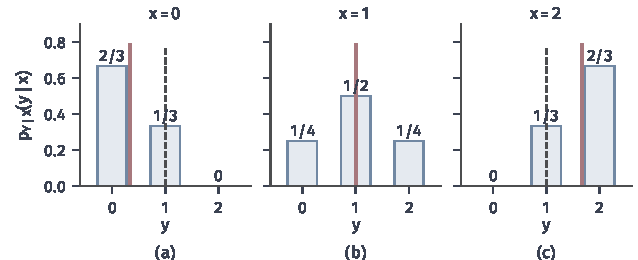
\includegraphics[width=108mm]{figures/07-probability/01-elementary-probability/matplotlib/rvc-conditional-pmf/figure.pdf}
  \caption{传感器表中给定第一台读数时第二台读数的条件分布。(a)、(b)、(c)分别对应$x=0,1,2$，柱高为$p_{Y\mid X}(y\mid x)$；红线是条件均值$1/3$、$1$、$5/3$，虚线是不加条件时的均值$1$。}
  \label{fig:rvc-conditional-pmf}
\end{BookInlineFigure}

把式~\eqref{eq:rvc-conditional-pmf}两边乘以$p_X(x)$，得到联合质量的另一种写法：
\begin{equation}
 p_{X,Y}(x,y)=p_X(x)\,p_{Y\mid X}(y\mid x).
 \label{eq:rvc-multiplication}
\end{equation}
它说明联合分布可以分两步给出：先按$p_X$定下$X$的值，再按该值对应的条件分布定下$Y$。许多模型正是这样描述的，先说明一个量怎样产生，再说明另一个量在前者给定时怎样产生。对$x$求和就是第~\ref{chap:classical-probability}章的全概率公式，
\[
 p_Y(y)=\sum_{x}p_X(x)\,p_{Y\mid X}(y\mid x),
\]
其中$p_X(x)=0$的项本来就是零，可以略去。反过来求给定$Y=y$时$X$的条件分布，就是Bayes公式：当$p_Y(y)>0$时，
\[
 p_{X\mid Y}(x\mid y)=\frac{p_X(x)\,p_{Y\mid X}(y\mid x)}{p_Y(y)}.
\]
传感器表关于对角线对称，例如$p_{X\mid Y}(0\mid 0)=0.3\cdot\frac23/0.3=\frac23$，与$p_{Y\mid X}(0\mid 0)$相同。

\paragraph{给连续变量取条件}
三角形模型中，若已知$X=0.6$，$Y$怎样分布？困难在于$\mathbb{P}(X=0.6)=0$，式~\eqref{eq:rvc-conditional-pmf}的分母为零。自然的办法是先以一个有正概率的窄带代替这个点：给定$x\leq X\leq x+h$，再让$h\to0$，见图~\ref{fig:rvc-conditional-slices}(a)。

设$f_{X,Y}$在$x$附近连续，且$f_X(x)>0$。窄带上的条件概率是两个积分之比，
\[
 \mathbb{P}(Y\leq y\mid x\leq X\leq x+h)
 =\frac{\int_{x}^{x+h}\int_{-\infty}^{y}f_{X,Y}(s,t)\,\mathrm{d}t\,\mathrm{d}s}{\int_{x}^{x+h}f_X(s)\,\mathrm{d}s}.
\]
分子分母同除以$h$。窄带越来越窄时，两者分别趋于被积函数在$s=x$处的值，于是
\[
 \lim_{h\to0}\mathbb{P}(Y\leq y\mid x\leq X\leq x+h)=\int_{-\infty}^{y}\frac{f_{X,Y}(x,t)}{f_X(x)}\,\mathrm{d}t .
\]
右边被积的函数正是窄带极限下$Y$的密度。

\begin{definition}[条件密度]
\label{def:rvc-conditional-density}
设$(X,Y)$有联合密度$f_{X,Y}$，$X$的边缘密度为$f_X$。对满足$f_X(x)>0$的$x$，定义
\begin{equation}
 f_{Y\mid X}(y\mid x)=\frac{f_{X,Y}(x,y)}{f_X(x)},
 \label{eq:rvc-conditional-density}
\end{equation}
称为给定$X=x$时$Y$的\term{条件密度}（conditional density）。
\end{definition}

和概率表一样，条件密度是联合密度沿竖线$\{X=x\}$的切片，除以切片的总积分$f_X(x)$而得到；它对$y$的积分为$1$。三角形模型中，对$0<x\leq1$有$f_X(x)=2x>0$，切片在$0\leq y\leq x$上取值$2$，所以
\[
 f_{Y\mid X}(y\mid x)=\frac{2}{2x}=\frac1x,\qquad 0\leq y\leq x .
\]
给定$X=x$时，$Y$服从$\operatorname{Unif}(0,x)$：均匀分布的点落在竖线上，只能落在三角形内的那一段，并且在这一段上没有偏好。

\begin{BookInlineFigure}
  \centering
  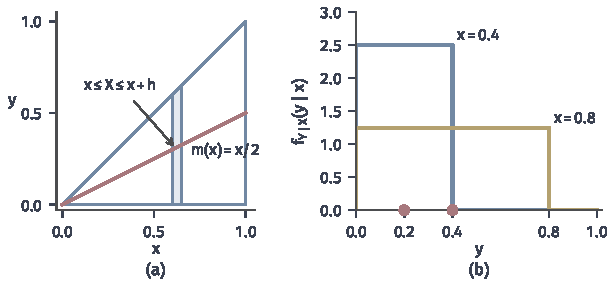
\includegraphics[width=104mm]{figures/07-probability/01-elementary-probability/matplotlib/rvc-conditional-slices/figure.pdf}
  \caption{三角形模型的条件化。(a)浅蓝窄带是事件$\{x\leq X\leq x+h\}$，$x=0.6$，$h=0.05$；红线是条件均值$m(x)=x/2$。(b)给定$X=0.4$（蓝）与$X=0.8$（黄）时$Y$的条件密度，分别是高$2.5$与$1.25$的矩形；红点是两个条件均值$0.2$与$0.4$。}
  \label{fig:rvc-conditional-slices}
\end{BookInlineFigure}

式~\eqref{eq:rvc-conditional-density}只在$f_X(x)>0$处使用。另一个限制更隐蔽：联合密度可以在一条竖线$\{x=x_0\}$上任意改动而不改变任何概率，改动后$f_{Y\mid X}(\cdot\mid x_0)$就变了。所以单独一个$x_0$处的条件密度并不由联合分布决定；只有把各个$x$处的条件密度合起来使用，例如对$x$积分，结果才有确定的意义。条件于零概率事件的严格含义，以及不同的取极限方式可能给出不同答案的现象，在第~\ref{chap:conditional-distributions}章说明。

有了条件密度，式~\eqref{eq:rvc-multiplication}和全概率公式都有连续版本：在$f_X(x)>0$处$f_{X,Y}(x,y)=f_X(x)f_{Y\mid X}(y\mid x)$，并且
\[
 f_Y(y)=\int f_X(x)\,f_{Y\mid X}(y\mid x)\,\mathrm{d}x,
\]
积分只在$f_X(x)>0$的范围进行。对三角形模型，$\int_{y}^{1}2x\cdot\frac1x\,\mathrm{d}x=2(1-y)$，与第~\ref{sec:rvc-joint}节直接求出的$f_Y$相同。

反方向的条件化同样计算。给定$Y=y$，$0\leq y<1$，由$f_Y(y)=2(1-y)>0$，
\[
 f_{X\mid Y}(x\mid y)=\frac{2}{2(1-y)}=\frac{1}{1-y},\qquad y\leq x\leq 1 ,
\]
即$X$在给定$Y=y$时服从$\operatorname{Unif}(y,1)$：较小的读数已知为$y$，较大的读数在$y$与$1$之间没有偏好。横线与竖线上的切片都是均匀的，但切片的位置与长度随条件改变，这正是两个分量不独立的表现。

\paragraph{条件分布与独立}
独立性可以换一种方式理解：知道$X$的值不改变$Y$的分布。在概率表的情形，由式~\eqref{eq:rvc-independence-pmf}与式~\eqref{eq:rvc-conditional-pmf}，$X,Y$独立当且仅当对每个满足$p_X(x)>0$的$x$，
\[
 p_{Y\mid X}(y\mid x)=p_Y(y)\quad\text{对一切}\ y\ \text{成立}.
\]
条件分布与$x$无关，各行重新归一以后长得一样。传感器表的三行形状各异，再次说明两台读数不独立。

有密度时，若$X,Y$独立，取$f_Xf_Y$为联合密度，条件密度就是$f_Y$，同样与$x$无关。图~\ref{fig:rvc-slices}比较了两个连续模型：$f=4xy$的条件密度在三个$x$处完全重合，都是$2y$；三角形模型的条件密度是宽度为$x$的矩形，随$x$改变。

\begin{BookInlineFigure}
  \centering
  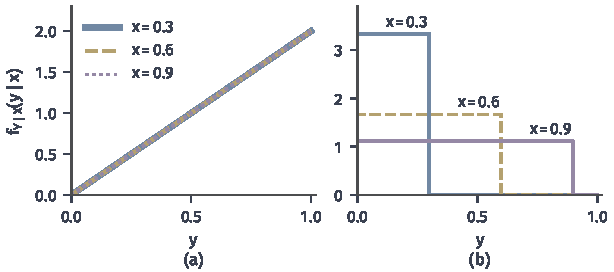
\includegraphics[width=104mm]{figures/07-probability/01-elementary-probability/matplotlib/rvc-slices/figure.pdf}
  \caption{独立就是条件分布不随条件改变。蓝、黄、紫分别对应$x=0.3,0.6,0.9$。(a)单位正方形上的密度$4xy$，三条条件密度重合为$2y$。(b)三角形模型，条件密度是$[0,x]$上高为$1/x$的矩形。}
  \label{fig:rvc-slices}
\end{BookInlineFigure}

\paragraph{离散状态与连续读数}
条件变量与被条件变量不必同属一类。设房间有两种状态：$X=0$表示正常，$X=1$表示过热，$\mathbb{P}(X=1)=0.2$。正常时一台精确传感器的读数$Y$服从$\mathcal{N}(20,1)$，过热时服从$\mathcal{N}(23,1)$。这里$X$有概率表，$Y$在给定$X$时有密度，联合规律由式~\eqref{eq:rvc-multiplication}的两步方式给出：
\begin{equation}
 \mathbb{P}(X=x,\,Y\in B)=p_X(x)\int_{B}f_{Y\mid X}(y\mid x)\,\mathrm{d}y .
 \label{eq:rvc-mixed-joint}
\end{equation}

对$x$求和，$Y$的边缘密度是两个高斯密度的加权和。记$\phi(z)=\mathrm{e}^{-z^{2}/2}/\sqrt{2\pi}$为标准高斯密度，则
\[
 f_Y(y)=0.8\,\phi(y-20)+0.2\,\phi(y-23).
\]
这种由若干分布按权重相加得到的分布称为\term{混合分布}（mixture distribution）。图~\ref{fig:rvc-mixture}(a)中，蓝线是$f_Y$，主峰来自正常状态，右侧的肩来自过热状态。

\begin{BookInlineFigure}
  \centering
  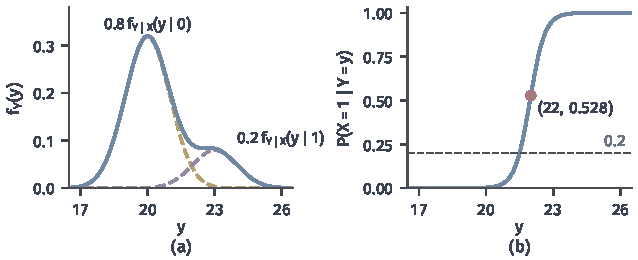
\includegraphics[width=108mm]{figures/07-probability/01-elementary-probability/matplotlib/rvc-mixture/figure.pdf}
  \caption{离散状态与连续读数。$\mathbb{P}(X=1)=0.2$，给定$X=0$与$X=1$时$Y$分别服从$\mathcal{N}(20,1)$与$\mathcal{N}(23,1)$。(a)蓝线为$Y$的密度，黄、紫虚线为两部分$0.8\,\phi(y-20)$与$0.2\,\phi(y-23)$。(b)读到$y$以后过热的条件概率，虚线是不加条件时的概率$0.2$，红点为$y=22$。}
  \label{fig:rvc-mixture}
\end{BookInlineFigure}

读到$Y=y$以后，过热的可能性有多大？$\mathbb{P}(Y=y)=0$，仍用窄带$y\leq Y\leq y+h$取极限，由式~\eqref{eq:rvc-mixed-joint}，分子分母同除以$h$后得到Bayes公式的密度形式：
\begin{equation}
 \mathbb{P}(X=1\mid Y=y)=\frac{p_X(1)\,f_{Y\mid X}(y\mid 1)}{f_Y(y)} .
 \label{eq:rvc-mixed-bayes}
\end{equation}
取$y=22$，两部分分别含$\phi(-1)$与$\phi(2)$，约去$1/\sqrt{2\pi}$，
\[
 \mathbb{P}(X=1\mid Y=22)=\frac{0.2\,\mathrm{e}^{-1/2}}{0.2\,\mathrm{e}^{-1/2}+0.8\,\mathrm{e}^{-2}}
 =\frac{1}{1+4\mathrm{e}^{-3/2}}\approx0.528 .
\]
读数$22$离过热状态的中心更近，过热的概率从$0.2$升到一半以上。取$y=21.5$时，两部分的指数相同，比值回到先验权重：$\mathbb{P}(X=1\mid Y=21.5)=0.2$，这个读数不提供区分两种状态的信息。

\paragraph{条件均值}
条件分布确定以后，可以像一元情形一样求它的期望。设$\mathbb{E}\lvert Y\rvert<\infty$，并且下面的和或积分有限，定义
\begin{equation}
 m(x)=\mathbb{E}[Y\mid X=x]=\sum_{y}y\,p_{Y\mid X}(y\mid x)\quad\text{或}\quad\int y\,f_{Y\mid X}(y\mid x)\,\mathrm{d}y ,
 \label{eq:rvc-conditional-mean}
\end{equation}
称为给定$X=x$时$Y$的\term{条件均值}（conditional mean）。它是“只看$X=x$那一组”时$Y$的平均，即组内平均。

传感器表中，由三行条件分布，
\[
 m(0)=\tfrac13,\qquad m(1)=1,\qquad m(2)=\tfrac53 ,
\]
可以合写为$m(x)=1/3+2x/3$。三角形模型中$Y$在给定$X=x$时服从$\operatorname{Unif}(0,x)$，$m(x)=x/2$。有趣的是，两个例子中$m$恰好都等于式~\eqref{eq:rvc-best-line}的最佳直线$\mu_Y+b^{*}(x-\mu_X)$：传感器表中$b^{*}=0.4/0.6=2/3$，三角形模型中$b^{*}=(1/36)/(1/18)=1/2$。一般情形下条件均值不必是直线，它作为最佳预测的含义在第~\ref{chap:conditional-expectation}章说明。

把$x$换成随机的$X$，得到随机变量$m(X)$，记作$\mathbb{E}[Y\mid X]$。它的值随$X$的值而定：传感器表中，$\mathbb{E}[Y\mid X]$以概率$0.3,0.4,0.3$取$1/3,1,5/3$。它的期望回到$Y$的期望，这就是下面的\term{全期望公式}（law of total expectation）。

\begin{theorem}[全期望公式]
\label{thm:rvc-total-expectation}
设$\mathbb{E}\lvert Y\rvert<\infty$，$X$有概率表或$(X,Y)$有联合密度。则
\begin{equation}
 \mathbb{E}[Y]=\mathbb{E}\bigl[\mathbb{E}[Y\mid X]\bigr]=\sum_{x}m(x)\,p_X(x)\quad\text{或}\quad\int m(x)\,f_X(x)\,\mathrm{d}x .
 \label{eq:rvc-total-expectation}
\end{equation}
\end{theorem}

\begin{proof}
在概率表的情形，由式~\eqref{eq:rvc-multiplication}，
\[
 \sum_{x}p_X(x)\,m(x)=\sum_{x}p_X(x)\sum_{y}y\,p_{Y\mid X}(y\mid x)=\sum_{x,y}y\,p_{X,Y}(x,y).
\]
条件$\mathbb{E}\lvert Y\rvert<\infty$保证二重和绝对收敛，求和可以按任意分组进行，右边就是$\mathbb{E}[Y]$。在密度的情形，把求和换成积分，并在$f_X(x)>0$处使用$f_{X,Y}=f_Xf_{Y\mid X}$。
\end{proof}

全期望公式就是“总平均等于各组平均的加权平均”，权重是各组的质量。传感器表中，
\[
 0.3\cdot\tfrac13+0.4\cdot1+0.3\cdot\tfrac53=0.1+0.4+0.5=1=\mathbb{E}[Y].
\]
三角形模型中，两个方向的条件均值分别是$m(x)=x/2$与$\mathbb{E}[X\mid Y=y]=(1+y)/2$，代入全期望公式，
\[
 \mathbb{E}[Y]=\frac{\mathbb{E}[X]}{2}=\frac13,\qquad \mathbb{E}[X]=\frac{1+\mathbb{E}[Y]}{2}=\frac23,
\]
都与边缘密度算出的结果一致。混合模型中$\mathbb{E}[Y]=0.8\cdot20+0.2\cdot23=20.6$。

\paragraph{全方差公式}
条件分布也有方差。设$\mathbb{E}[Y^{2}]<\infty$，在概率表的情形定义
\begin{equation}
 v(x)=\operatorname{Var}(Y\mid X=x)=\sum_{y}\bigl(y-m(x)\bigr)^{2}p_{Y\mid X}(y\mid x),
 \label{eq:rvc-conditional-variance}
\end{equation}
称为给定$X=x$时$Y$的\term{条件方差}（conditional variance）；密度的情形把和换成积分。它是组内的散开程度。$Y$的总方差与它有什么关系？回答是下面的\term{全方差公式}（law of total variance）。

\begin{theorem}[全方差公式]
\label{thm:rvc-total-variance}
设$\mathbb{E}[Y^{2}]<\infty$，$X$有概率表或$(X,Y)$有联合密度。则
\begin{equation}
 \operatorname{Var}(Y)=\mathbb{E}\bigl[v(X)\bigr]+\operatorname{Var}\bigl(m(X)\bigr).
 \label{eq:rvc-total-variance}
\end{equation}
\end{theorem}

\begin{proof}
记$\mu_Y=\mathbb{E}[Y]$，在概率表的情形证明。固定满足$p_X(x)>0$的$x$，把$y-\mu_Y$拆成$(y-m(x))+(m(x)-\mu_Y)$，在条件分布下求平方的平均。交叉项含有$\sum_{y}(y-m(x))p_{Y\mid X}(y\mid x)$，由$m(x)$的定义它等于零，于是
\[
 \sum_{y}(y-\mu_Y)^{2}p_{Y\mid X}(y\mid x)=v(x)+\bigl(m(x)-\mu_Y\bigr)^{2}.
\]
两边乘以$p_X(x)$再对$x$求和。由式~\eqref{eq:rvc-multiplication}，左边成为
\[
 \sum_{x,y}(y-\mu_Y)^{2}p_{X,Y}(x,y)=\operatorname{Var}(Y).
\]右边第一项是$\mathbb{E}[v(X)]$；由全期望公式$\mathbb{E}[m(X)]=\mu_Y$，第二项是$\operatorname{Var}(m(X))$。密度的情形逐字把求和换成积分。
\end{proof}

证明中的第一个等式是力学中的平行轴定理：质量对任意一点的二阶矩，等于对自身重心的二阶矩加上重心偏移的平方。式~\eqref{eq:rvc-total-variance}于是读作：总波动等于组内波动的平均，加上各组平均之间的波动。

三个例子逐一核对。传感器表中三行的条件方差为$2/9,1/2,2/9$，$m(X)=1/3+2X/3$，所以
\[
 \mathbb{E}[v(X)]=0.3\cdot\tfrac29+0.4\cdot\tfrac12+0.3\cdot\tfrac29=\tfrac13,\qquad
 \operatorname{Var}\bigl(m(X)\bigr)=\bigl(\tfrac23\bigr)^{2}\cdot0.6=\tfrac{4}{15},
\]
两者之和为$9/15=0.6=\operatorname{Var}(Y)$。三角形模型中$v(x)=x^{2}/12$，$m(X)=X/2$，
\[
 \mathbb{E}[v(X)]=\frac{\mathbb{E}[X^{2}]}{12}=\frac{1}{24},\qquad
 \operatorname{Var}\bigl(m(X)\bigr)=\frac{\operatorname{Var}(X)}{4}=\frac{1}{72},
\]
和为$1/18$。混合模型中两组的方差都是$1$，组平均$20$与$23$以权重$0.8,0.2$分布，组间方差为$3^{2}\times0.8\times0.2=1.44$，所以$\operatorname{Var}(Y)=1+1.44=2.44$。

由式~\eqref{eq:rvc-total-variance}，$\mathbb{E}[v(X)]\leq\operatorname{Var}(Y)$：平均而言，知道$X$以后$Y$的不确定性不会增加。但这只对平均成立，个别条件可以让波动变大。单位圆盘的均匀分布中，$\operatorname{Var}(Y)=\mathbb{E}[Y^{2}]=1/4$，而给定$X=0$时$Y$服从$\operatorname{Unif}(-1,1)$，条件方差为$1/3$；圆盘中央那条竖线比整个圆盘在竖直方向更“长”。

本节的计算都针对给定的具体取值$x$，结果是$x$的普通函数。把条件均值当作随机变量来研究，例如它为什么是在已知$X$时对$Y$的最佳预测、在什么意义下唯一，属于第~\ref{chap:conditional-expectation}章；没有概率表也没有密度时怎样定义条件分布，属于第~\ref{chap:conditional-distributions}章。


\section{本章小结}
\label{sec:rvc-summary}

本章从两台传感器的问题出发：两台同时报偏高的概率、一台读数已知时另一台的规律、平均以后的波动，都要求知道几个量在同一次观测中怎样共同取值。把定义在同一样本空间上的随机变量排成随机向量，这份共同规律就是联合分布。离散时它是一张概率表，连续时是单位面积上的质量即联合密度，两类模型都可以用联合分布函数描述，矩形概率由四个角上的值确定。

从联合分布出发，本章得到的几种对象可以放在同一张概率表上看。表~\ref{tab:rvc-summary}按传感器表列出它们的算法与结果。

\begin{BookInlineTable}
  \centering
  \caption{从联合分布得到的对象（传感器表）}
  \label{tab:rvc-summary}
  \begin{tabular}{lll}
    \toprule
    对象 & 在概率表上的操作 & 结果 \\
    \midrule
    边缘分布 & 按行、按列求和 & $(0.3,0.4,0.3)$ \\
    独立性 & 每格与边缘之积比较 & 不独立 \\
    均值向量 & 按质量加权平均 & $(1,1)^{\top}$ \\
    协方差 & 中心化乘积加权求和 & $0.4$ \\
    条件分布 & 取出一行，除以行和 & 如$(\tfrac23,\tfrac13,0)$ \\
    条件均值 & 对每行求均值 & $\tfrac13+\tfrac23x$ \\
    \bottomrule
  \end{tabular}
\end{BookInlineTable}

边缘化把其余分量的信息汇总掉，不能逆转：相同的边缘可以对应许多不同的联合分布。只有在独立时，联合分布才由边缘拼成乘积；判别时，概率表要求每个格子分解，密度要求边缘乘积本身就是联合密度。独立带来两项计算上的便利：乘积的期望可以分开计算（两个期望有限时），条件分布不随条件改变。独立同分布同时要求同分布与相互独立，两项不能互相替代；两两独立也不足以推出相互独立。

均值向量是质量分布的重心，协方差矩阵描述质量沿各个方向的散开程度。它对称半正定，$\bm{a}^{\top}\bm{\Sigma}\bm{a}$是$\bm{a}^{\top}\bm{X}$的方差，奇异时质量压在一个超平面上。有限和的方差展开中，交叉项来自分量之间的协方差，它决定平均能把波动降低多少：各读数方差同为$\sigma^{2}$、两两相关系数同为$\rho>0$时，无论平均多少个读数，方差都降不到$\rho\sigma^{2}$以下。相关系数介于$-1$与$1$之间，衡量向一条直线集中的程度；独立推出不相关，反之不成立，零相关只排除线性关联。

条件分布在概率表中是取出一行再重新归一，在密度中是取一条切片再除以$f_X(x)$，只在分母为正时使用。条件均值是组内平均，全期望公式说总平均是组平均的加权平均，全方差公式把总方差分成组内方差的平均与组平均之间的方差。单个零概率条件下的条件密度不由联合分布唯一确定，严格的处理在第~\ref{chap:conditional-distributions}章完成。

下一章用这些结构考察具体的多元模型：多项计数的和为常数，造成奇异协方差；多元高斯分布由均值向量和协方差矩阵完全确定；共同尺度可以让不相关的分量仍然相互依赖。按给定联合分布实际产生样本以及效率问题，在第~\ref{chap:sample-generation}章展开。

